\section{Introduction} \label{sec:intro}
Breadth-first search (BFS) is the basic building component of many graph algorithms 
and is thus of vital importance to high-performance graph processing. Nevertheless, 
it is notoriously difficult for accelerating on FPGAs because of the 
irregular memory access and the low computation-to-memory ratio. 
At the same time, BFS on large graphs also involves tremendous 
parallelisms which indicate great potential for acceleration. 
With both the challenge and the parallelization potential, 
BFS has attracted a number of researchers exploring its acceleration on FPGAs 
\cite{attia2014cygraph, betkaoui2012reconfigurable, Dai2017foregraph, Ma2017fpga,
umuroglu2015hybrid, oguntebi2016graphops, engelhardt2016gravf, zhou2016high}. 

Previous work have shown that BFS accelerators on FPGAs can provide competitive  
performance and superior energy efficiency when given comparable memory bandwidth. 
However, these work typically optimize BFS or relatively general graph processing 
with dedicated circuit design using hardware description language (HDL). The HDL 
based designs with customized circuits are beneficial to the resulting performance 
and save resource consumption, but it usually takes long time for development, 
upgrade, maintenance and porting to a different FPGA device, which are all 
important concerns from the perspective of the accelerator developers. Another 
engineering yet non-trivial problem is the high barrier to use the FPGA powered graph 
processing accelerators in high-level applications such as 
big data analytics, which is mostly caused by the lack of 
well-defined high level interface and user-friendly SDK supporting 
various hardware systems. Improving the ease of using the 
HDL based accelerators requires a lot of design efforts 
such as driver and runtime environment to support newer 
devices and diverse computing systems. This is also one of 
the key obstacles hindering the widespread adoption of 
the FPGA accelerators despite the great performance-energy 
efficiency advantages.

The limitation of the conventional HDL design method in combination with the 
rapid advancements of the HLS techniques makes the HLS tools attractive. 
HLS tools are increasingly adopted in both industry and academia for rapid FPGA prototyping and 
application acceleration. Software programmable FPGAs \cite{koch2016fpgas, xilinx-sdaccel} 
gets widespread acceptance. Nevertheless, the current HLS based design tools are mostly used for 
applications with relatively regular memory access patterns and data paths. 
It remains challenging for the HLS tools to accelerate BFS with irregular 
memory access patterns and complex data paths. In general, the main reasons lies in the 
following aspects. First of all, the HLS tools nowadays can support only very limited 
on-chip buffer optimizations, so it is rather difficult to handle irregular memory accesses 
especially random memory accesses. Secondly, hardware pipelining strategy in HLS tools 
is usually conservative to ensure the functional correctness, while 
this also leads to inefficient hardware implementations when the data path is data 
dependent or dynamic. Under such a context, we explore the use of Intel OpenCL for 
efficient BFS acceleration on software programmable FPGAs.

To cope with the irregular memory accesses and dynamic data paths in BFS, we proposed 
a series of optimization methods to regularize 
both the data path and memory accesses for efficient HLS implementation. 
We start with graph edge reordering. Basically, the edges 
are shuffled based on its destination vertices and divided into batches. In each batch, 
the edges point to different segments of the vertices. Then we have the vertex visiting 
status stored into multiple on-chip buffer banks while each bank stores the visiting status 
of vertices in different vertex segments. In combination with the edge batching, we can read 
and process the edges in the granularity of batches without any stall. In addition, we also have 
the coupled CPU to gather the scattered frontier vertices' edge location and union them as 
as an sequential array such that the data path on the FPGA can be pipelined smoothly. 
According to the experiments on a set of big graphs, the optimized high level BFS 
accelerator achieves up to 70X performance speedup when compared to the design 
in Spector benchmark. It achieves around 80\% of the handcrafted design on 
similar FPGA boards. 

The major contributions of this work are summarized as follows.
\begin{itemize}
    \item As far as we know, this is the first highly optimized and open-sourced 
		HLS based BFS accelerator on FPGAs targeting portability and ease of 
		use on top of performance. 
    \item We proposed a set of combined methods to regularize the irregular
		memory accesses and dynamic data paths of BFS. This may shed light on similar 
		irregular application acceleration on FPGAs using HLS tools.
    \item The resulting accelerator shows significant performance speedup 
        over a baseline HLS design and gets close to state-of-art handcrafted 
		design on a set of representative graphs.
\end{itemize}

The rest part of the paper is organized as follows. In Section \ref{sec:relatedwork}, 
we brief the background of software programmable FPGAs and related work of 
BFS acceleration especially on FPGAs. In Section \ref{sec:motivation},  
we analyze the performance of basic BFA implementations with best-effort HLS 
optimizations and demonstrate the challenge of BFS acceleration using OpenCL. 
In Section \ref{sec:bfs-opt}, we present the overview of the BFS accelerator 
design using OpenCL and detail the major optimization methods.
In Section \ref{sec:experiment}, we present comprehensive experiments of the 
BFS accelerator. Finally, we conclude this work in Section \ref{sec:conclusion}.

\section{Background and related work} \label{sec:relatedwork}
In this section, we briefly introduce the high level FPGA design tools.
Then we review the existing BFS acceleration work and introduce the widely 
used BFS algorithm for the BFS accelerator design.

\subsection{High level FPGA design tools}
HDL based FPGA design is mostly limited to 
highly skilled hardware designers and hinders 
the adoption of FPGAs in more domains of applications.
In addition, the HDL based design typically results in low design productivity, 
large reuse, portability and maintenance cost as well 
as ease of use challenge. 
To address this problem, the FPGA vendors have started 
to offer high level programming options such as C/C++ and OpenCL, which makes 
it possible for the designers without much low-level circuit design 
experiences \cite{nimbix, xilinx-sdaccel, intel-opencl} 
to program the FPGAs efficiently. In addition, the accelerator 
described with high level languages preserves many software-like features 
such as portability, ease of maintenance and use. They are all 
important concerns from the perspective of the designers. Considering the  
continuously increasing FPGA resources and stringent time-to-market requirements, 
the high level FPGA design tools \cite{Nane2016hls-survey} are getting more and more 
popular.

In line with this trend, we use SDAccel \cite{xilinx-sdaccel} to develop the 
high level BFS accelerator in this work. SDAccel overview is presented in 
Figure \ref{fig:sdaccel}. It is a design environment targeting x86-Based server + PCIe 
based FPGA acceleration card. Compared to the conventional design flow, it provides 
a number of features to make the FPGAs programmable to software designers. 
First of all, it allows the designers to implement the computing kernel with either 
C/C++ based HLS or OpenCL. The designers can further optimize the kernel with 
corresponding pragmas such as loop unrolling and pipelining. Secondly, it allows the 
designers to perform fast software emulation with which debugging, function verification 
as well as some preliminary profiling of the kernel can be done rapidly.
Finally, the compute kernel is wrapped as an OpenCL thread. With the provided libraries, it 
can be referenced through the standard OpenCL API in high level applications conveniently.
With this reason, the same design can be seamlessly 
ported to other FPGAs with SDAccel support including the FPGAs in 
Xilinx Nimbix Cloud \cite{nimbix}.     

\begin{figure}
\center{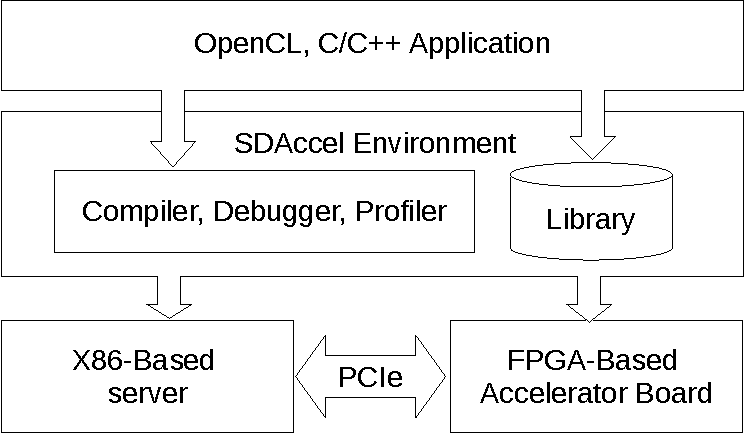
\includegraphics[width=0.75\linewidth]{sdaccel}}
    \caption{Xilinx SDAccel design framework \cite{xilinx-sdaccel}}
\label{fig:sdaccel}
\end{figure}

\subsection{BFS Algorithm}
BFS is a widely used graph traversal algorithm and it is the basic 
building component of many other graph processing algorithms. 
It traverses the graph by processing all vertices with the same distance from the 
source vertex iteratively. The set of vertices which have the same distance from the 
source is defined as frontier. The frontier that is under analysis in the BFS iteration 
is named as current frontier while the frontier that is inspected from current frontier 
is called next frontier. By inspecting only the frontier, BFS can be implemented efficiently 
and thus the frontier concept is utilized in many BFS implementations.

BFS algorithm can be formalized as follows. Assume $G$ is a graph with vertex 
set $V$ and edge set $E$, BFS finds a shortest path from a source vertex
$v_s \in V$ to all the other vertices in the graph $G$. For each vertex $v \in V$, 
BFS will output a level value $l$, indicating its distance from $v_s$ ($v$ can be accessed 
from $v_s$ by traveling through $l - 1$ edges. 

A widely used frontier based BFS algorithm implementation is named as 
level synchronous BFS \cite{attia2014cygraph, betkaoui2012reconfigurable, 
zhang2017boosting}. The details of the algorithm are presented in 
Algorithm \ref{alg:level-bfs}.
The basic idea is to traverse the frontier vertices and inspect the neighbors 
of the current frontier vertices to obtain the frontiers in next BFS iteration. 
Then the algorithm can start a new iteration with a simple switch of 
current frontier queue and next frontier queue. The algorithm ends when 
the frontier queue is empty.

\begin{algorithm}
    \small
	\caption{Level Synchronous BFS Algorithm} \label{alg:level-bfs}
	\begin{algorithmic}[1]
		\Procedure{BFS}{}
		\State $level[v_k] \gets -1$ where $v_k \in V$
		\State $level[v_s] \gets 1$
		\State $current\_frontier \gets v_s$
		\State $current\_level \gets 1$
		\While {$current\_frontier$ not empty} 
		\For{$v \in current\_frontier$}
		\State $S \gets {n \in V | (v, n) \in E}$
		\For {$n \in S$}
		\If {$level[n] == -1$}
		\State $level[n] \gets current\_level + 1$
		\State $next\_frontier \gets n$
		\EndIf
		\EndFor
		\EndFor
		\State $current\_level \gets current\_level + 1$
		\State Swap $current\_frontier$ with $next\_frontier$
		\EndWhile
		\EndProcedure
	\end{algorithmic}
\end{algorithm}

\subsection{Related work}
The growing importance of efficient BFS traverse on large graphs 
have attracted attentions of many researchers. In the past few years, 
many BFS optimization algorithms and accelerators have been proposed 
on almost all the major computing platforms including multi-core processors, 
distributed systems, GPUs and FPGAs. In this work, we will 
particularly focus on the FPGA based BFS acceleration. 

The researchers tried to explore BFS acceleration 
on FPGAs from many various angles.
To alleviate the memory bandwidth bottleneck of the 
BFS accelerators, the authors in \cite{zhang2017boosting} 
explored the emerging Hybrid Memory Cube (HMC) which provides 
much higher memory bandwidth as well flexibility for BFS 
acceleration, while the authors in \cite{attia2014cygraph} 
proposed to change the compressed sparse row (CSR) format slightly. 
Different from the first two work, the authors in \cite{umuroglu2015hybrid} 
choosed to perform some redundant but sequential memory access for higher memory bandwidth 
utilization based on a spare matrix-vector multiplication model.
In addition, they particularly took advantage of the 
hybrid CPU-FPGA architecture offloading only highly parallel 
BFS iterations for FPGA acceleration while leaving the rest 
on host CPU.  

Most of the BFS accelerators are built on a vertex-centric 
processing model, while the authors 
in \cite{zhou2016high} explored the edge-centric graph processing and demonstrated 
significant throughput improvement. On top of the single FPGA board acceleration, 
the authors in \cite{attia2014cygraph, betkaoui2012reconfigurable} also explored 
BFS acceleration on a FPGA based high performance computing system with multiple 
FPGAs and memory instances. There are also work exploring customized soft processors 
for graph processing and building a distributed solution on 
top of a group of embedded FPGA boards \cite{kapre2015custom, wang2010message}.

Instead of building specialized BFS accelerator, many researchers opted to develop 
more general graph processing accelerator framework or library 
recently \cite{engelhardt2016gravf, oguntebi2016graphops, Dai2017foregraph, dai2016fpgp}. 
They can also be utilized for BFS acceleration despite the lack of 
specialized optimization for BFS. Meanwhile, this is also a way to improve 
the ease of use FPGAs for graph processing acceleration.

Prior BFS acceleration work have demonstrated the potential benefits of accelerating 
BFS on FPGAs. These accelerators were mainly developed for the sake 
of performance and generality for more graph processing algorithms. 
However, they were all handcrafted HDL designs. Developing the HDL based accelerators 
takes long time and applying these accelerators 
on high level applications for software designers still requires a lot of 
efforts especially when the target computing platforms are different. 
To that end, we opt to develop HLS based BFS accelerators 
using SDAccel such that the accelerator packed in an 
OpenCL thread can be easily utilized in high level applications 
by a \textit{software designer}. Meanwhile, the same design can be easily 
ported to other FPGAs with the SDAccel support with negligible 
engineering efforts.

\section{Observations on BFS memory access} \label{sec:observation}
BFS on large graphs is known to be a memory bandwidth bound task.
Thus we analyze the memory access of BFS for intensive optimization. 
With the analysis, three observations are gained and can be used to 
guide the BFS accelerator design.

\textit{Observation 1: BFS memory access pattern  
involves considerable short sequential memory accesses 
and random memory accesses which are usually quite 
expensive. At the same time, it also includes quite some long 
sequential memory accesses and the overall access time can't be 
ignored due to the relatively large memory access amount.} We analyze the 
memory access pattern of the BFS on Youtube Graph. The burst length distribution 
of the memory accesses is presented in Figure \ref{fig:burst-len-youtube}. 
(In FPGA design, longer sequential memory access can be usually taken as burst 
transfer from the perspective of an internal bus. We use 
the burst and sequential access interchangeably in this paper.)
It can be found that there are a large amount of random and short sequential 
memory access. Meanwhile, we notice that shorter burst length especially 
the random memory access results in extremely low memory bandwidth 
when compared to that of longer sequential memory access. Worse still, 
more parallel data paths with the typical data width i.e. 32-bit will 
not improve the memory bandwidth utilization too much due to the memory 
access conflict, which makes the random and short sequential 
memory access optimization difficult. Note that the memory bandwidth is obtained 
from a separate HLS based memory test on an Alpha Data ADM-PCIE-7v3 FPGA card.
We use the test result to estimate the memory access time of BFS. 
In general, it can be concluded that the short sequential and random 
memory access are the most critical part of the BFS memory accesses. 
 
\begin{figure}
\center{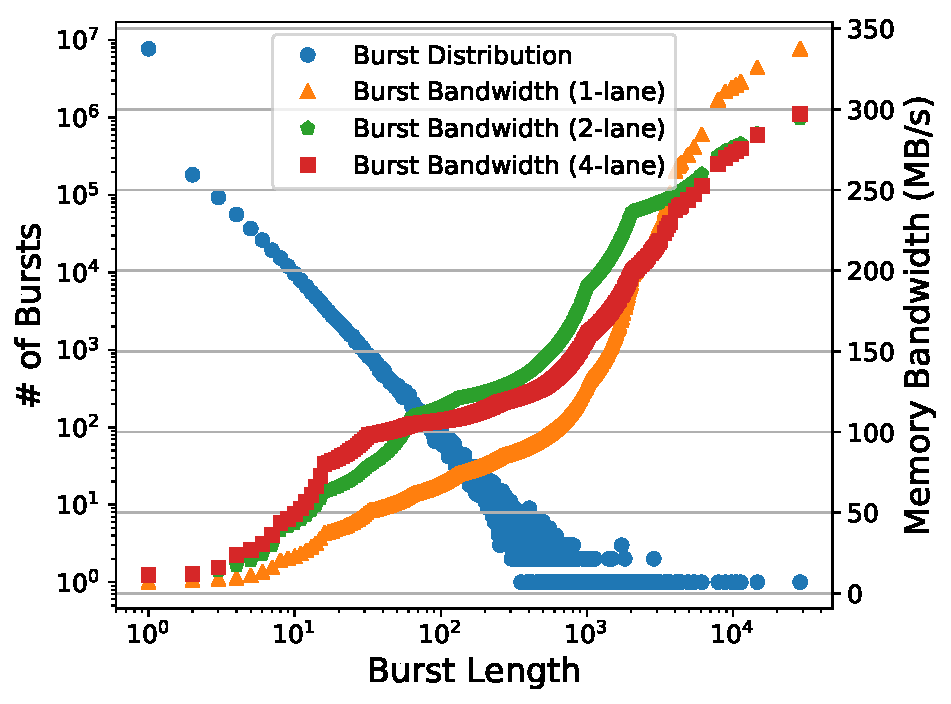
\includegraphics[width=0.85\linewidth]{burst_len_youtube}}
\caption{Burst length distribution in BFS on Youtube Social Network Graph. 
    Random memory access and short sequential memory access take up the 
    the majority of the memory access overhead of BFS. Multiple parallel 
    lanes of data paths improve the memory bandwidth utilization when the 
    burst lenght is relatively large, but they will not help much 
    for short or random memory accesses.}
\label{fig:burst-len-youtube}
\end{figure}

\textit{Observation 2: There are many redundant vertices in the 
frontier vertex neighbors leading to a lot of redundant memory access in BFS.} 
As random memory access takes up a big portion of the overall memory 
access overhead, we further investigate the random memory access in BFS. 
According to the level synchronous BFS algorithm, the random memory access mainly comes 
from the frontier neighbor vertex status read/write. 
However, many frontier vertices may have common neighbor vertices and these common 
vertices lead to many repeated vertex status read. To gain insight of the neighbor 
vertex redundancy, we compare the total amount of frontier 
neighbor vertices and the amount of unique frontier neighbor vertices in each BFS iteration.
(Note that we use the Youtube graph as an example in the experiment as well.) 
The comparison is shown in Figure \ref{fig:repeat-neighbor} and it can be clear 
that there are a lot of redundant vertices in most of the BFS iterations. 
The redundancy proportion even goes up to 80\% in the BFS iteration with the most frontiers. 
With proper redundancy removal strategy, the vertex status reads in the following 
part of the BFS can be reduced dramatically.

On top of the redundant vertices, the visited vertices in previous 
BFS iterations don't need to be checked by reading the vertex status 
from memory. According to our experiment, the visited frontiers 
take up quite some of the total frontier neighbor vertices. However, this is 
observed in only one or two BFS iterations. Buffering 
frontier vertices may help to avoid unnecessary random vertex status read, 
but the benefit may be relatively trivial.  

\begin{figure}
\center{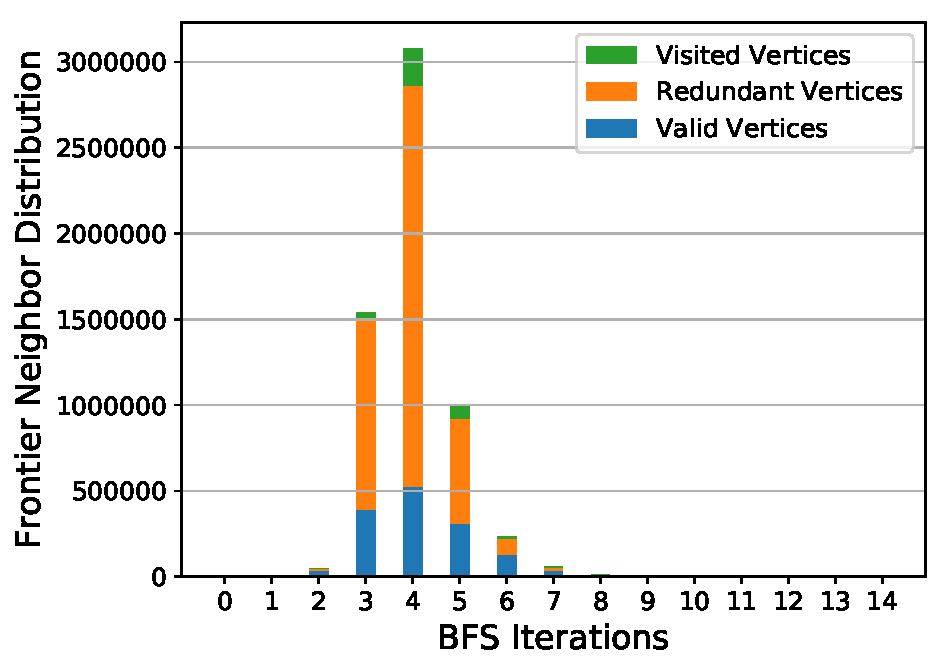
\includegraphics[width=0.85\linewidth]{neighbor_vertex}}
\caption{Unnecessary random vertex status read decomposition. 
    The frontier neighbors consists of three parts including visited vertices 
    in previous BFS iterations (visited vertices), 
    redundant vertices that are repeatedly traversed in one BFS iteration (redundant vertices), 
    and the actual valid vertices that must be traversed (valid vertices). 
    The first two parts of the vertices can be ignored without 
    affecting the correctness of the BFS.}
\label{fig:repeat-neighbor}
\end{figure}

\textit{Observation 3: The vertex status reads have good 
spatial locality especially when the redundant access are removed in advance, 
but the temporal locality is relative bad meaning that the status reuse 
distance is quite long.}
Another potential optimization of random memory access is to use cache architecture, 
which explores the data locality and improves memory bandwidth utilization 
accordingly. To ascertain the feasibility of using cache, we analyze both the 
temporal and spatial locality of the vertex status reads. Since 
the frontier neighbor vertex redundancy removal affects the locality, 
we also do the spatial locality analysis on a redundancy-free 
vertex status read sequence. The data locality based cumulative 
distribution function (CDF) curve is shown in 
Figure \ref{fig:youtube-locality}. Clearly the memory accesses exhibit 
very good spatial locality. In particular, the spatial 
locality gets even better and over 70\% of the vertices have reference distance 
less than 200 when the redundancy is squeezed. The temporal locality is not as 
good and only around 20\% of the accesses have short reuse distance. In general, 
we still believe that a specialized cache is beneficial to the random 
vertex status reads. Note that we use 
the stride distance as the metric of spatial locality and reuse distance as the metric 
of temporal locality \cite{weinberg2008chameleon}. The stride distance of a reference 
to address A is defined as the minimum distance between A and the 
memory addresses in a lookback window right before the current 
memory access. We set the loopback window to be 32 in the experiment. 
The reuse distance of some reference to 
address A is equal to the number of unique memory addresses that have been 
accessed since the last access to A.  

\begin{figure}
\center{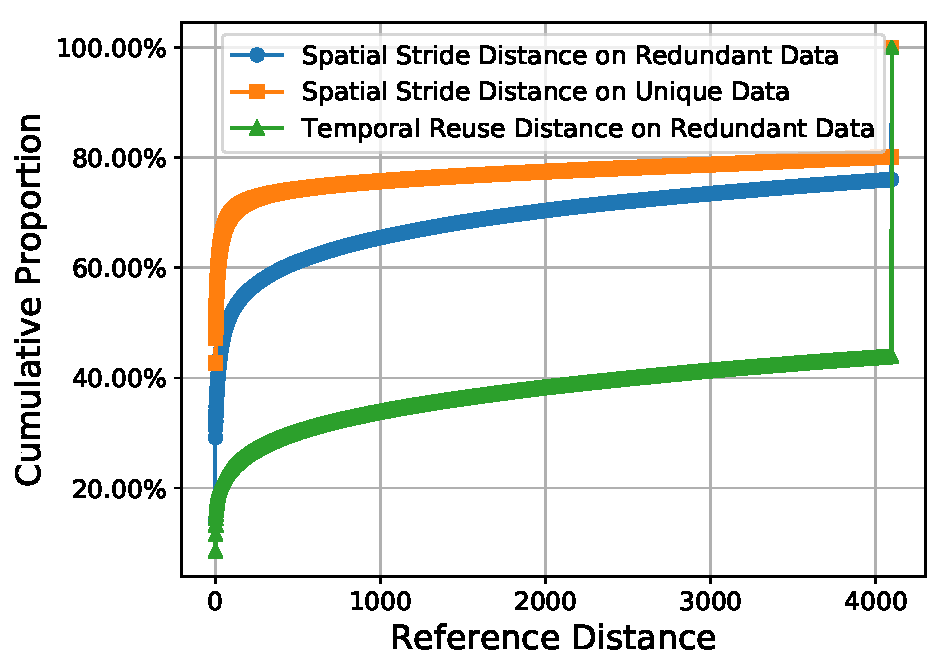
\includegraphics[width=0.8\linewidth]{youtube-locality}}
\caption{Cumulative Distribution Function (CDF) of reuse distance 
    and stride distance. They stand for the temporal locality and spatial 
    locality of the BFS vertex status reads respectively. Note that the 
    accesses with reference distance larger than 4000 are combined as they are difficult 
    to be optimized in hardware design.}
\label{fig:youtube-locality}
\end{figure}

%\textit{Observation 4: In the skewed graphs, a small amount of high degree vertices 
%covers a big proportion of the connections (edges) in the graph.}
%The real-world graphs usually have large amount of vertices and adges while 
%the FPGA on chip memory is far from enough for caching and buffering. 
%Hereby, only a sub set of them can reside in on-chip memory at runtime. 
%It can be expected that high degree vertex related information 
%are more likely to be referenced in 
%the BFS iterations. To further investigate the potential of buffering 
%the high degree vertices, we analyzed the vertex degree distribution 
%of Youtube graph. The vertex degree based CDF and vertex based 
%CDF is shown in Figure \ref{fig:degree-distribution}. The two CDF curves in the figure 
%exhibit that the top 10\% high degree vertices include more than 70\% of 
%vertex degree namely edges in the graph. Basically keeping these high degree 
%vertex infomration such as vertex status on chip can avoid the repeated 
%vertex staus checking in BFS and is benefitial to the memory access efficiency. 
%Another thing that is worth for highlighting is the one degree vertex distribution.
%It takes up over 40\% of the overall amount of the vertices in the graph. In BFS, 
%the status of these vertices will be read and write only once.  
%
%\begin{figure}
%\center{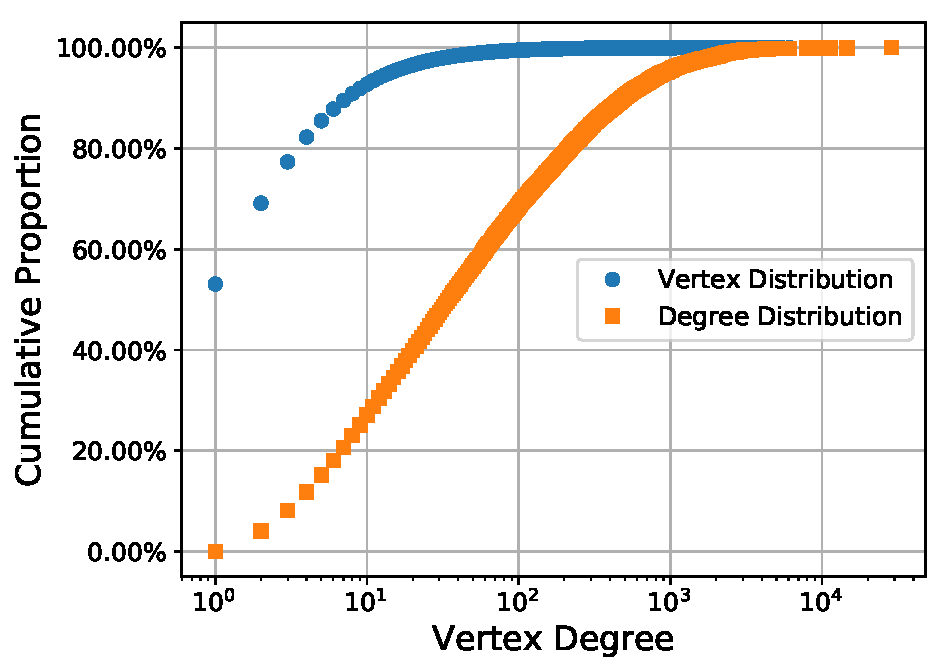
\includegraphics[width=0.9\linewidth]{degree-dist}}
%\caption{Vertex Degree Distribution. A small amount of 
%    high degree vertices take up a large portion of the connections in the graph.}
%\label{fig:degree-distribution}
%\end{figure}

In summary, we notice that random and short sequential memory accesses 
are the most time-consuming part of the overall BFS memory accesses. 
It is generally difficult to optimize these memory accesses, 
With intensive experiments, we observe large amount of redundancy in BFS and 
these memory accesses exhibit very good spatial locality. Taking advantage of the 
memory access characteristics, we may optimize the BFS memory access efficiency 
and improve the BFS performance eventually.

\section{BFS Accelerator Overview} \label{sec:overview}
Figure \ref{fig:accelerator-overview} presents the overview of 
the BFS accelerator. It targets in-memory graphs on a PCIe based 
high performance FPGA card. The whole graph is stored in FPGA device 
memory with a standard CSR format. 
Ideally, the accelerator does the BFS on FPGA without 
any interference from the host CPU. However, we organize the accelerator 
following the data flow model of Xilinx HLS and the data flow model 
doesn't allow feedback from the downstream stages to previous stages.
(Detailed BFS data flow will be illustrated in the next section.)
As a result, we can only put one BFS iteration on FPGA while 
leaving the iterative execution control to the host CPU. In each BFS iteration, 
the BFS kernel on FPGA returns the BFS frontier size to host such that the host will 
decide if another BFS iteration should be invoked. Although short communication 
between the host and FPGA in each BFS iteration is needed, the communication cost 
is negligible compared to the execution time. Hereby, 
the overall BFS runtime is barely affected.

\begin{figure}
\center{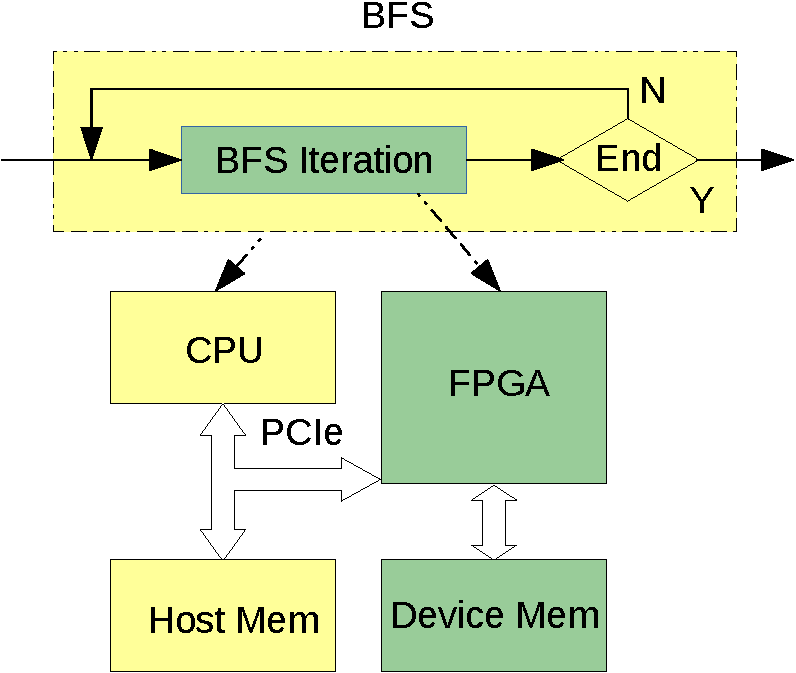
\includegraphics[width=0.6\linewidth]{accelerator-overview}}
\caption{BFS accelerator overview}
\label{fig:accelerator-overview}
\end{figure}

The BFS algorithm is critical to the BFS accelerator and we explore the 
existing level synchronous BFS algorithm in detail. We notice that 
the level synchronous BFS algorithm may have redundant vertices pushed to the 
frontier queue in a parallel architecture especially when the frontier grows larger.
The main reason roots in the large amount of overlapped neighbor vertices among the 
frontier vertices as mentioned in previous section. When the frontier neighbors 
are inspected in parallel for faster BFS traverse, these overlapped vertices may be 
considered as frontiers independently and inserted into the next frontier queue. 
As a result, there may be redundant vertices put into the frontier queue and it is 
rather complex to get rid of the redundancy \textit{completely}. Although the redundant 
vertices in the frontier will not cause any BFS mistakes, they will soon lead to large 
amount of redundant traverses recursively and degrade the BFS performance.

To address this problem, we analyze the frontier from the 
vertex status in each BFS iteration to completely cut down the 
propagation of the redundant frontier vertices as proposed in prior 
GPU based BFS acceleration \cite{liu2015enterprise}. The modified algorithm is described 
in Algorithm \ref{alg:modified-bfs}. Instead of inspecting on the frontier vertices directly, 
it starts with vertex status analysis and inspects the frontier 
in each BFS iteration. Although it seems the additional frontier inspection stage 
brings more memory access, the inspection processing are complete sequential 
memory access and can be done efficiently. It is still worth for the overhead 
when compared to the cost caused by the redundant frontier vertices. 
The rest part of the algorithm from line 10 to 15 is 
quite similar to the level synchronous BFS except that the frontier queues 
are no longer needed.

\begin{algorithm}
	\caption{Modified BFS Algorithm} \label{alg:modified-bfs}
    \small
	\begin{algorithmic}[1]
		\Procedure{BFS}{}
		\State $level[v_k] \gets -1$ where $v_k \in V$
		\State $level[v_s] \gets 0$
		\State $current\_level \gets 0$
		\State $frontier \gets v_s$

        \While {$!frontier.empty()$} 

		\For{$v \in V$}
		\If{$level[v] == current\_level$}
		\State $frontier \gets v$
		\EndIf
		\EndFor

		\For{$v \in frontier$}
		\State $S \gets {n \in V | (v, n) \in E}$
		\For {$n \in S$}
		\If {$level[n] == -1$}
		\State $level[n] \gets current\_level + 1$
		\EndIf
		\EndFor
		\EndFor
		\State $current\_level \gets current\_level + 1$
		\EndWhile
		\EndProcedure
	\end{algorithmic}
\end{algorithm}

\section{HLS based BFS optimization} \label{sec:bfs-opt}
With the observations in Section \ref{sec:observation} 
and the modified BFS algorithm in Section \ref{sec:overview}, 
we start to optimize the BFS accelerator using high level design tools 
from a series of different angles. First of all, we convert the nested loop structure 
of the BFS to be a stream manner such that it can be fit into the data flow model in
Xilinx HLS for efficient pipelined execution. Then we explore a series of memory optimization 
techniques based on the BFS memory access characteristics observed in \ref{sec:observation}. 
Afterwards, we further apply some general HLS optimizations to the resulting design. Finally, 
we manually tune the design parameters such as the prefetch buffer size and cache size through 
the fast software emulation and provide optimized configurations for each graph data set.

\subsection{BFS pipelining}
The baseline BFS algorithm is a multi-level nested loop with 
dynamic memory accesses. It is quite challenging for the HLS 
tools to produce optimized hardware by adding the HLS pragmas to 
the native high level code directly because of the following two 
reasons. First of all, inner most loop and outer loop body can't be pipelined 
automatically by the HLS tools unless the inner most loop is fully 
unrolled and pipelined. Nevertheless, the inner most loop in BFS 
can't be fully unrolled because of the dynamic loop structure.  
Secondly, the outer loop nests access memory randomly even though 
these accesses are actually sequential because they must wait 
for the execution of the inner loop nest which can't 
be fully pipelined. This will lead to low 
memory bandwidth utilization. Similar problem also happens when the 
loop body is complex and different parts of the loop body fail to be 
pipelined properly. In summary, applying HLS pragmas to the native high level BFS code 
will produce low efficient design and the performance of the resulting hardware 
can be far from satisfying.  

To address these problems, we divide the BFS algorithm into pipelined 
sub functions. Basically, there are generally two rules that 
we can create pipelined functions. 
First of all, each loop nest can be packaged into a sub function 
and the dependent sub functions can be pipelined. There are four loop 
nests in Algorithm \ref{alg:modified-bfs}, 
but the loop in line 12 actually include two loops as we need to go through 
both the CSR row and column to obtain a frontier neighbor's index. Thus we 
actually have five sub functions following this rule. Secondly, complex loop body 
can be split to more fine-grained sub functions such that the dependent parts can 
be executed in parallel with additional buffers between them. 
In BFS inner most loop, we can further divide the \textit{depth} read and write 
operations to two dependent sub functions. We can 
do more partitions and create even deeper pipelines, while there is no 
guarantee for always better performance and more hardware resources 
are usually required.

Following the two pipelining rules, we create a six-stage 
pipelined BFS algorithm as detailed in Algorithm \ref{alg:bfs-stream}. 
The six sub functions are labeled as f1 to f6 respectively. In f1, 
vertex status is read from FPGA DDR memory sequentially through a streaming port. 
When the vertex status is fetched, f2 inspects the status 
flowed from the stream buffer, decides the current frontier 
and dumps the frontier to the downstream pipeline. 
With the frontier stream, f3 can further fetch graph 
data stored as CSR. CSR includes a row pointer array (RPA) 
and a column index array (CIA), and they must be sequentially accessed. 
In f3, we combine each pair of RPA entry of the frontier as a construct 
and pass it to the next stream function f4. When f4 gets the RPA pair, 
it can read the CIA sequentially through a streaming port. 
When data in CIA stream which is essentially the potential 
next frontier vertices are received in f5, their vertex status 
will be checked by reading the vertex status array stored in DDR as well.
Only the vertices that are not visited yet will be further forwarded to the f6. 
In f6, the vertex status will be updated.

\begin{algorithm}
	\caption{Pipelined BFS Algorithm} \label{alg:bfs-stream}
    \small
	\begin{algorithmic}[1]
        \Procedure {BFS}{}
        \State $frontier\_size \gets 1$
        \State $level \gets 0$
        \While {$(frontier\_size > 0)$}
        \State $f1(depth, depth\_stream)$
        \State $f2(depth\_stream, frontier\_stream, level, frontier\_size)$ 
        \State $f3(frontier\_stream, CSR.RPA, RPA\_stream)$
        \State $f4(RPA\_stream, CSR.CIA, CIA\_stream)$ 
        \State $f5(CIA\_stream, depth, next\_frontier\_stream)$
        \State $f6(depth, next\_frontier\_stream, level)$
        \State $level \gets level + 1$
        \EndWhile
        \EndProcedure
        \State

        \Procedure{f1}{$depth$, $depth\_stream$}
        \For {$v \in V$}
        \State $depth\_stream << depth[v]$
        \EndFor
        \EndProcedure

        \Procedure{f2}{$depth\_stream, frontier\_stream, level, frontier\_size$}
        \State $frontier\_size = 0$
        \For {$v \in V$}
        \State $d[v] \gets depth\_stream.read()$
        \If {$(d[v] == level)$}
        \State $frontier\_stream << v$
        \State $frontier\_size++$
        \EndIf
        \EndFor
        \EndProcedure

        \Procedure{f3}{$frontier\_stream, CSR.RPA, RPA\_stream$}
        \While {$(!frontier\_stream.empty())$}
        \State $v \gets frontier\_stream.read()$
        \State $RPA\_stream << [CSR.RPA[v], CSR.RPA[v+1]]$
        \EndWhile
        \EndProcedure

        \Procedure{f4}{$RPA\_stream, CSR.CIA, CIA\_stream$}
        \While {$(!RPA\_stream.empty())$}
        \State $[begin, end] \gets RPA\_stream.read()$
        \For {${v \in CSR.CIA(begin, end)}$}
        \State $CIA\_stream << v$
        \EndFor
        \EndWhile
        \EndProcedure

        \Procedure{f5}{$CIA\_stream, depth, next\_frontier\_stream$}
        \While {$(!CIA\_stream.empty())$}
        \State $v \gets CIA\_stream.read()$
        \If {$(depth[v] == -1)$}
        \State $next\_frontier\_stream << v$
        \EndIf
        \EndWhile
        \EndProcedure

        \Procedure{f6}{$depth, next\_frontier\_stream, level$}
        \While {$(!next\_frontier\_stream.empty())$}
        \State $v \gets next\_frontier\_stream.read()$
        \State $depth[v] \gets level + 1$
        \EndWhile
        \EndProcedure

    \end{algorithmic}
\end{algorithm}

According to the description of the streamed BFS algorithm, we notice that 
five sub functions involve external memory access and they have quite different 
memory access patterns. The memory access patterns are summarized in 
Figure \ref{fig:bfs-stream}. f3 reads all the vertex status and 
it has a long sequential memory read. f2 reads the CSR row pointer of the frontier, 
and it reads two sequential words each time. f1 reads the CSR column index and the 
burst length depends on the vertex degree which varies in a large range. 
f4 and f5 involves vertex status reads and writes of the next frontier vertices.
As these vertices are not sequential, the HLS tools just take them as random access 
without any specific hints from the designers. 

\begin{figure}
\center{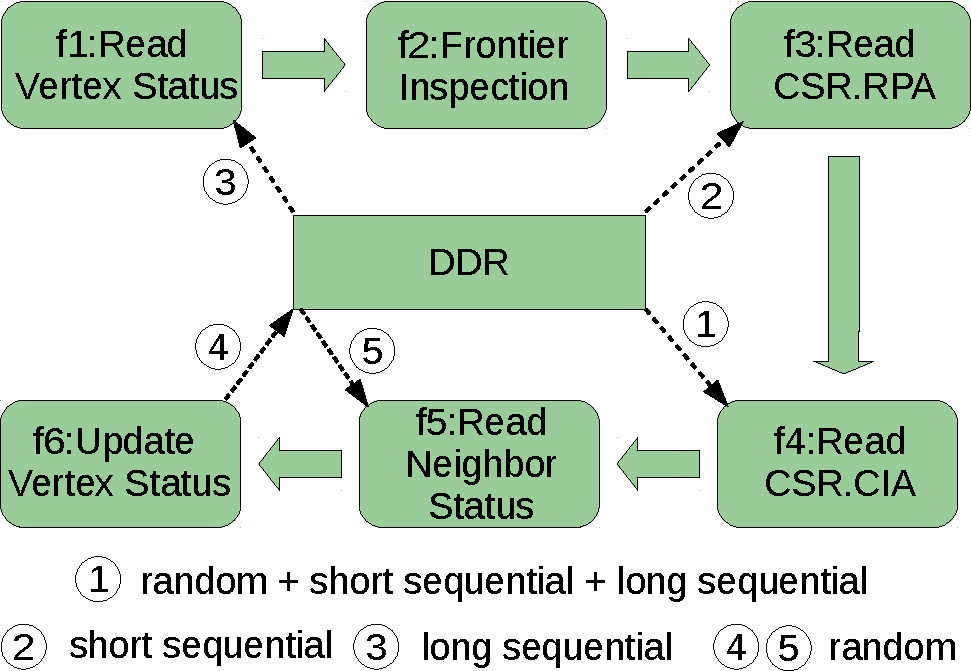
\includegraphics[width=0.65\linewidth]{bfs-stream}}
\caption{Streamed BFS Algorithm}
\label{fig:bfs-stream}
\end{figure}

\subsection{Memory Access Optimization}
As observed in Section \ref{sec:observation}, memory access especially the random and 
short sequential memory accesses are critical to the 
BFS performance. In this sub section, we will mainly explore the memory 
access optimization techniques based on the observations on top of 
the pipelined BFS design.

\subsubsection{Redundancy Removal}
There are many redundant vertices among the frontier neighbors in BFS. 
They may further cause unnecessary vertex status reads and writes in 
f5 and f6 respectively. In order to remove the redundant memory access 
and improve the memory bandwidth utilization, we create hash tables 
to perform the redundancy removal. As the redundant vertices are 
relatively random, a big hash table can be utilized to squeeze 
the redundancy. However, big hash table degrades the hardware implementation 
frequency and eventually lowers the overall performance. Hereby, we 
build a series of smaller hash tables and apply them in parallel. 
The hash table based redundancy removal structure is shown in Figure \ref{fig:hash-strategy}. 
We use the lower bits of the data address as the hash function 
for the sake of better timing. An input data that fails to find a 
record in any of the hash tables will be considered to be a unique 
data and put into one of the hash tables to avoid repeated data 
going through the filter. In order to ensure balanced hash 
table utilization, we implement a hardware-friendly round robin 
arbiter to decide the hash table updating order. 
  
\begin{figure}
\center{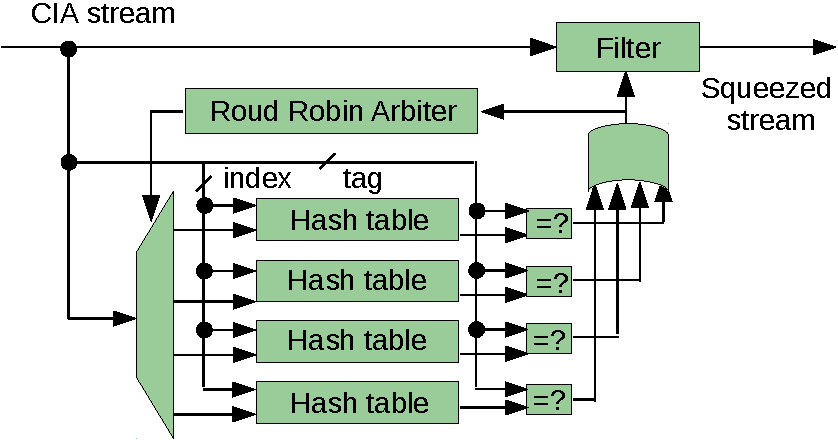
\includegraphics[width=0.75\linewidth]{hash-strategy}}
    \caption{Redundancy removal based on parallel hash tables.}
\label{fig:hash-strategy}
\end{figure}

\subsubsection{Caching}
According to the experiments in Section \ref{sec:observation}, 
there are many random memory accesses and short 
sequential memory accesses in f5 and f6. 
It is generally difficult to optimize these memory accesses. Fortunately, 
the spatial locality analysis shown in the observation experiments 
implies the great potential of cache based memory access optimization. 
Inspired by the observation, we developed an HLS based cache specifically 
for the vertex status \textit{depth} access. 

Since the cache is only used for \textit{depth} array read and write, we  
choose the \textit{depth} array index instead of its physical address for cache 
indexing. Each cache line is set to be 512-bit which is equal to the recommended 
memory access data width and a single memory read or write operation can 
fulfill the requirement of the cache operations including cache read miss, 
cache write miss and cache write back. Since the cache can't be shared 
between different SDAccel data flow functions, a natural cache design is 
to implement both cache in f5 and f6. Both cache can be relatively simple 
for supporting only read operations in f5 and write operations in f6.  

In this work, we choose the directly mapped cache for the BFS optimization. 
Cache line size is set to be 64B which fits well with the optimized global memory 
access port data width.
Although set associative cache architectures will achieve higher 
cache hit rate, the benefit is mostly compromised by the degraded 
implementation frequency on Alpha Data FPGA board. The trade-off 
may be different on a more advanced FPGA boards, but the optimization 
philosophy is pretty much similar. 
 
\subsubsection{Prefetching}
According to the BFS algorithm, the frontier is sequentially inspected. 
Therefore, the CSR information is also accessed in one direction 
in f3 and f4, though they are not necessarily sequential. Basically 
both the column array index and the row column index will increase 
monotonically in one BFS iteration. The CSR data will not be repeatedly 
referenced through the BFS. To optimize these memory 
accesses, a small prefetch buffer 
is build to improve the memory access efficiency. 

Prefetch buffer is also an important design parameter that needs to be tuned.
The general design trade-off is complex.
A larger prefetch buffer improves the hit rate, but it may incur more memory 
access cost and waste the memory bandwidth if the prefetched data are 
not fully used. Meanwhile, larger prefetch buffer adds prefetching cost 
when there is prefetch buffer miss, which may degrade the performance. 
A smaller prefetch buffer typically lead to lower hit rate though 
the prefetched data will be mostly used. Nevertheless, we notice that 
prefetching data that is smaller than 64B will not have clear advantages on timing 
nor memory bandwidth utilization compared to 64B prefetch buffer. 
On the other hand, prefetching more than 64B data doesn't have 
significant hit rate improvement and even results in 
performance drop mainly due to the increase of the prefetch cost when there 
is prefetch buffer miss. In this case, 64B is set to be the prefetch buffer size 
in the end.

\subsection{General HLS optimization}
On top of the pipelining, redundancy removal and caching, there are also 
many other relatively general design optimizations that can improve the 
resulting BFS accelerator performance. These optimizations will be briefly 
introduced in this sub section.

\subsubsection{Data path duplication}
When the DDR memory bandwidth is not saturated, a simple 
yet efficient optimization method is to duplicate the data paths. 
With multiple parallel BFS data paths, the accelerator can issue more parallel 
memory requests pushing higher memory bandwidth utilization. A straightforward 
way of data path duplication is to split the vertex status into different 
partitions and each partition is processed by an instance of the same BFS data path.

However, this method may not work as good as expected for three reasons. 
First of all, the vertices in the frontier may not distribute evenly across the graph. 
As a result, the different pipelines may have unbalanced workloads. Secondly, 
when the cache is applied to the pipelined data path, the same cache line may 
have multiple copies stored in f6 cache and this may cause 
cache coherence problem when they are modified differently 
and written back to memory independently. Finally, duplicating 
the non-bottleneck pipeline stages will not be beneficial to 
the final performance while it incurs more hardware resource consumption 
including not only the basic FPGA cells but also the global memory ports. 

To address the problems, we propose a delicate data path duplication strategy 
as shown in Figure \ref{fig:duplicate-pipeline}. According to the BFS algorithm, 
we know that each frontier vertex requires two CSR row pointer read and multiple 
CSR column index read. Thus the bottleneck pipeline stages may probably start 
from f3. In this case, we split the stream generated in f3 into 
multiple streams. Each sub stream will be handled independently by a 
duplicated data path. This also solves the data path load balancing problem 
naturally. Finally, to ensure a simple yet efficient cache coherence, we 
merge the output stream of f5 into a single stream before flowing into the 
last f6 stage with a write cache. 

\begin{figure}
\center{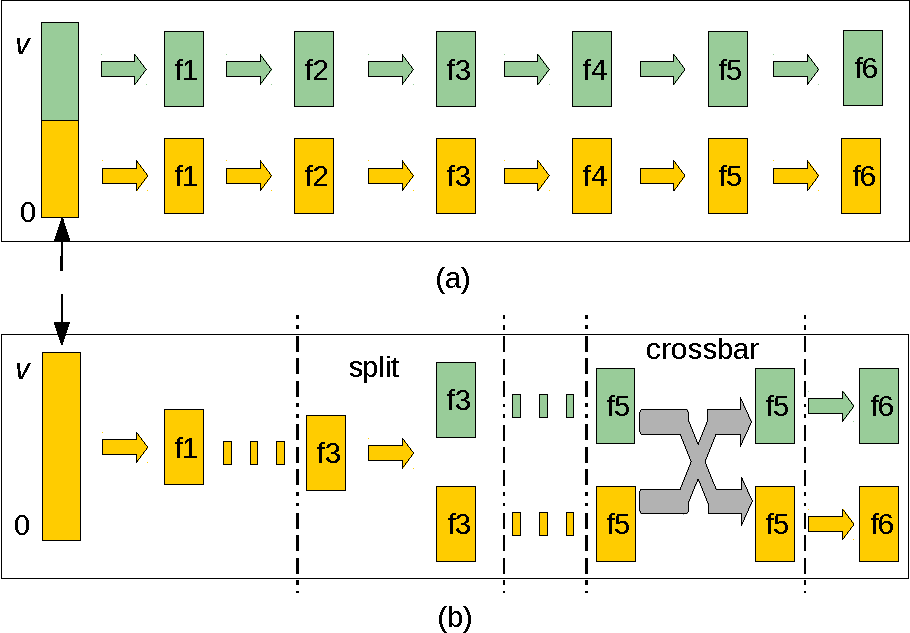
\includegraphics[width=0.85\linewidth]{pipeline-duplication}}
    \caption{pipeline duplication. (a) straightforward pipeline duplication 
    (b) optimized pipeline duplication.}
\label{fig:duplicate-pipeline}
\end{figure}


\subsubsection{Data width optimization}
The memory bandwidth utilization is sensitive to the data width setup. 
According to our experience, sequential memory access 
with 512-bit data width achieves the optimal memory bandwidth. With this guideline, 
a lot of design parameters such as the cache line size and prefetch length are 
set to be 512-bit for higher memory bandwidth utilization. For sequential 
memory access with smaller data width such as 32-bit, we must ensure that the 
data is aligned to 512-bit through padding the access. Otherwise, writing 
unaligned data may corrupt the data in memory.

%\subsubsection{II optimization}
%In the pipelined design, initialization interval (II) indicates the 
%processing throughput. Larger II in a single pipeline stage 
%may slow down the rest of the system. Thus we try to reduce II of all 
%the pipelined sub functions. In particular, hash table, cache and prefetch 
%buffer may affect the II. Inappropriate implementation may lead to 
%large II and even compensate the benefits brought by these optimizations. 

\subsubsection{Deadlock removal}
Another challenge of the pipelined BFS accelerator design is the 
unexpected deadlock problem. 
When a pipeline stage issues a long burst request to the memory 
but gets stalled due to the insufficient read buffer, it has to 
wait for the downstream pipeline stages to consume the data in the buffer. 
However, the downstream pipeline stages may also be stalled due to 
the failure of acquiring the bus that is taken by the upstream pipeline stage.
It is difficult to debug and resolve this deadlock. To address this problem, we
add additional user buffer in the pipeline stages with long sequential 
memory access and split the long sequential memory access into smaller 
segments such that each segment can be accommodated by the buffer. 
Although this may cause slightly lower bandwidth utilization, it breaks the deadlock and 
ensures the correctness of the pipelined design.

\subsection{Parameter Tuning}
As presented in previous sub sections, there are quite some design 
parameters such as hash table size and cache design, 
that need to be explored. However, exploring the design parameters 
based on the hardware implementation directly requires many lengthy 
hardware implementations (A typical BFS implementation may 
take 1 hour to 4 hours to complete.) which is extremely time-consuming.

In this work, we manually tune the design paramters. To obtain the optimized 
design parameters rapidly, we extract a series of hardware implementation independent 
metrics such as cache hit rate and hash table hit rate 
through faster software emulation mode in SDAccel which typically completes in a few minutes.
With these metrics, we can roughly decide the prefetch buffer size, 
cache size and hash table size etc. Afterwards, we go through the lengthy 
hardware implementation and choose the best parameters based on the final 
run time. A more systematic design parameter tuning will be helpful, but it 
is beyond the scope of this work and we will leave it for our future work.

%\subsection{Parameter tuning}
%In this work, we manually tune the design parameters. To obtain the 
%optimized design parameters rapidly, we proposed a general HLS design 
%parameter tuning flow for the HLS based design. The design flow is 
%presented in Figure \ref{fig:parameter-tuning}. It includes three 
%iterative loops tuning different types of the design parameters.
%
%The first loop replies on the fast software emulation which is 
%immediately available using HLS.
%With the software emulation, we can extract a set of statistical 
%metrics such as cache hit rate, prefetch hit rate that are 
%mostly independent with the hardware implementation. These metrics can be used to 
%guide the cache and prefetch buffer design. Although they 
%are not sufficient to decide the exact accelerator performance, they 
%can help prune the design options that are far from optimal and thus reduce 
%the design parameter tuning time. The second tuning loop is based on the hardware 
%pre-synthesis which is also fast and can be done in a few minutes. 
%With the pre-synthesis report, we can optimize the II by 
%improving the HLS design. When the potential design 
%configurations gets smaller, we can get into the last loop and start the time consuming 
%hardware implementation evaluating the configurations with the real 
%performance or resource metrics. Finally, we would like to emphasize the verification process, 
%it needs to be enabled all the time, as optimization may also cause mistakes of the resulting design.
%
%\begin{figure}
%\center{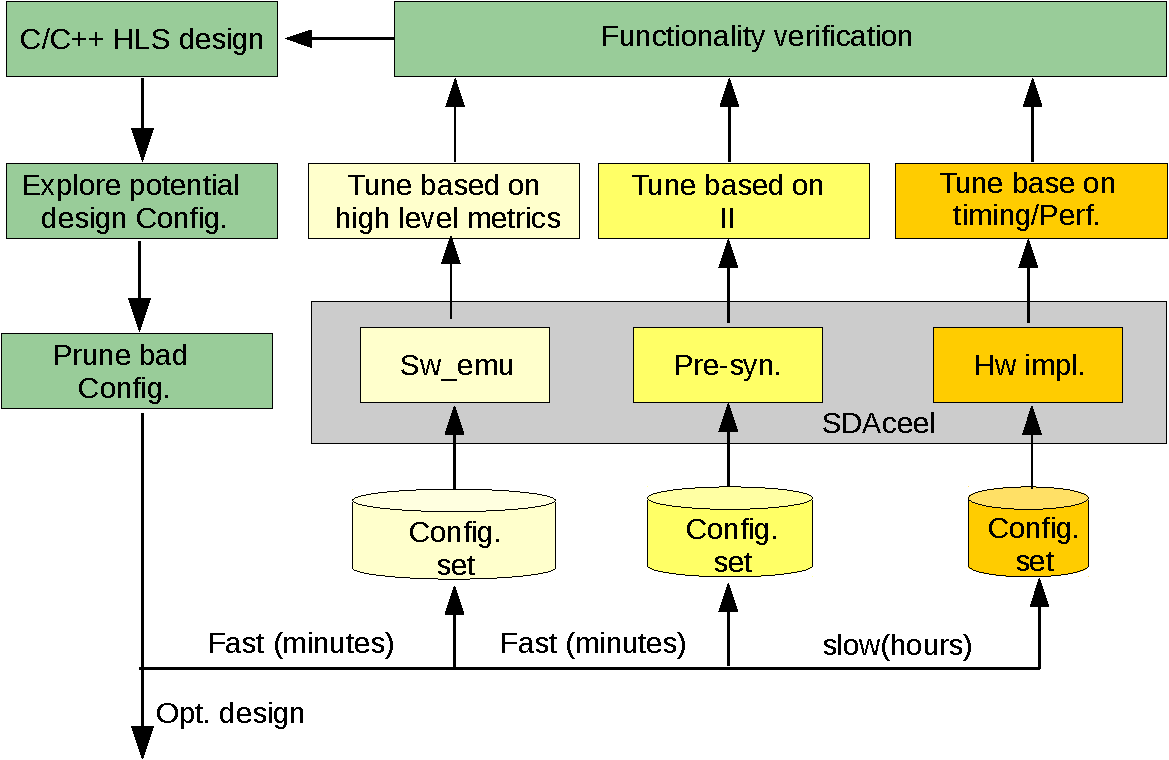
\includegraphics[width=0.95\linewidth]{parameter-tuning}}
%    \caption{Design parameter tuning flow based on SDAccel.}
%\label{fig:parameter-tuning}
%\end{figure}
%

%\appendix
%\section{Acknowledgement}

%\begin{acks}
%  The authors would like to thank Sam Ho for providing the suggestions on
%  HLS design debugging and optimization as well as the SDAccel usage. 

%\end{acks}
